%\item Interpretation of results
The results described above do not present clear evidence that the Reggio Approach is an effective early childhood program. However, there are several considerations of the evaluation context and the data that we expand upon here. We consider the possibility that it is possible that over time, the programs grew to share more features. Because this means that the Reggio Approach and the alternatives are more similar along some dimensions, this would reduce the estimated treatment effects of the Reggio Approach.\footnote{See \citet{Elango_Hojman_etal_2016_Early-Edu} for a discussion of considering the counterfactual in early childhood education evaluations.} In order to understand the trajectory of the programs, we wrote a survey to structure interviews with key individuals in the different school systems of Reggio Emilia, Parma, and Padova (see Appendix~\ref{sec:survey} for a full description of the survey and its implementation). We asked if the schools had aspects that are also present in the Reggio Approach schools, as well as details about their specific programs. These key aspects that make up the Reggio Approach were collected from published materials as well as confirmed by staff of the Reggio Approach. 

We present the similarities and differences between the different programs in Figures~\ref{fig:agg-admin} and~\ref{fig:agg-ped}. Using results from the structured interviews, we compute the number of administrative and pedagogical components that each program shares with the Reggio Approach by school type, city, and year. We examine 14 administrative components and 12 pedagogical components. Over time, many of the programs other than the state programs, adopt more features present in the Reggio Approach. This is especially true of the Parma municipal program. This supports the claim that the alternative schools and the Reggio Approach schools evolved to share more characteristics.

\begin{figure}[H]
\begin{center}
\begin{subfigure}[b]{0.55\textwidth}
	\caption{Number of Administrative Characteristics in Common with the Reggio Approach}\label{fig:agg-admin}
	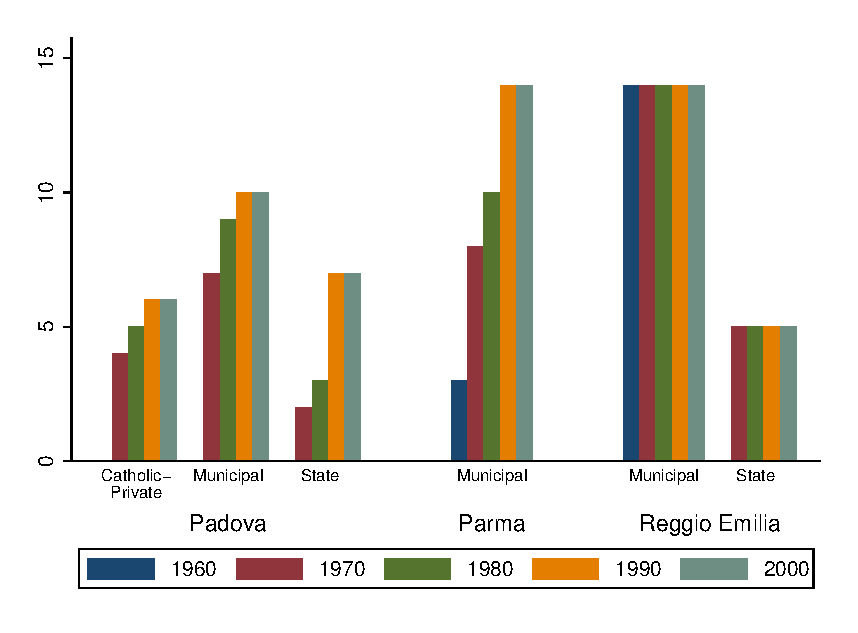
\includegraphics[width=\textwidth]{../../output/aggregateAdministrative.eps}
\end{subfigure}%
~
\begin{subfigure}[b]{0.55\textwidth}
	\caption{Number of Pedagogical Characteristics in Common with the Reggio Approach}\label{fig:agg-ped}
	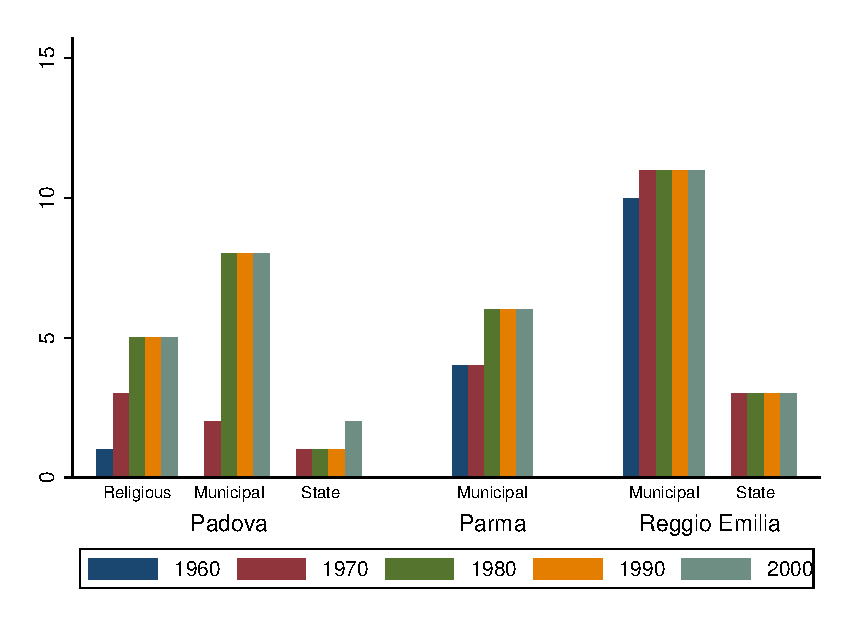
\includegraphics[width=\textwidth]{../../output/aggregatePedagogical.eps}
\end{subfigure}%
\end{center}
\raggedright \footnotesize Note: These graphs show the number of administrative and pedagogical components that each program has in common with the Reggio Approach. We consider 14 administrative components and 12 pedagogical components. One of the pedagogical components, following a set curriculum, was not present in the Reggio Approach. 
\end{figure}

% more details on survey results

%\item Expand discussion of survey highlighting specific questions that presented interesting results
In addition to this historical context, we expand on shortcomings in the data that make more precise analysis difficult. It is clear that selection into the Reggio Approach is an important factor to consider. We presented estimates with different control sets to better understand the importance of observed background characteristics that can determine this selection. Controlling for more background characteristics, especially in the younger cohorts, makes the treatment effects more positive. With more precise background variables, such as a more complete variable for family income, we could better capture the disadvantage in the sample, allowing our estimates to be less biased. More background variables for the older cohorts would be especially useful considering there were fewer available for them.

%In Appendix~\ref{appendix:mlogit} we present the results from the multinomial logit model, which gives the marginal effect that a background characteristic has on attending a certain type of preschool arrangement.

Other variables would allow other analysis that attempts to account for differential selection on background characteristics. Although we attempted to construct instruments for enrollment, including distance to the nearest school and the presence of a grandparent nearby, these variables proved to be poor instruments, and not available for the older cohorts. Variables capturing the selection apart from background characteristics, such as complete tuition costs, would provide the opportunity to implement another specification to compute the treatment effects.

%\begin{itemize}
%	\item Discuss differences in eligibility requirements between cities and schools and how that might have contributed to differential selection
%	\item Data issues
%\end{itemize}


